\chapter{Studi Literatur}

\par Pada bab ini dipaparkan hasil studi literatur terkait dengan kompetisi \textit{competitive programming}. Studi literatur yang dilakukan adalah terkait sistem yang digunakan dalam menyelenggarakan kompetisi \textit{competitive programming}, \textit{online judging system}, \textit{autograder} dan metode yang digunakan dalam melakukan grading.

\section{\textit{Competitive Programming}}

\par \textit{Competitive programming} merupakan sebuah kompetisi dimana peserta dari kompetisi tersebut diminta menyelesaikan suatu permasalahan pada bidang \textit{computer science} secara cepat dan tepat. Pada kompetisi \textit{competitive programming}, peserta akan diberikan permasalahan \textit{computer science} yang sudah pernah diselesaikan dan bukan permasalahan riset yang solusinya masih belum ditemukan (\cite{halimsfcp3}). Untuk setiap persoalan yang diberikan, peserta diminta untuk menyelesaikan masalah tersebut dengan membuat program dalam bahasa pemrograman yang diizinkan oleh juri. Program yang dibuat oleh peserta harus memenuhi batasan yang dibuat oleh juri seperti waktu eksekusi, kebutuhan memori, dan ukuran program.
\par Pada kompetisi \textit{competitive programming}, program yang telah dibuat oleh peserta akan dinilai dengan suatu metode tertentu. Umumnya penilaian yang dilakukan mencakup kebenaran program dan waktu pengumpulan program, akan tetapi terdapat beberapa metode penilaian lain yang dapat dilakukan. Beberapa standar metode telah digunakan untuk melakukan penilaian jawaban dalam kompetisi \textit{competitive programming}, diantaranya adalah standar IOI dan ICPC. Beberapa kompetisi \textit{competitive programming} diselenggarakan oleh suatu organisasi, contohnya adalah ICPC yang diselenggarakan oleh ICPC Foundation (\cite{abouticpc}), dan IOI (International Olympiad in Informatics) yang diselenggarakan oleh IOI Community (\cite{ioiorg}). Selain itu, terdapat juga kompetisi \textit{competitive programming} yang diselenggarakan oleh suatu perusahaan seperti Google Code Jam yang diselenggarakan oleh Google dan Facebook HackerCup yang diselenggarakan oleh Facebook.
\par Kompetisi \textit{competitive programming} pada tingkat perguruan tinggi biasanya mengikuti standar ICPC. Beberapa kompetisi yang mengikuti standar ini antara lain adalah Gemastik, Compfest, Vocomfest, INC, dan ACM-ICPC. Pada standar ICPC, setiap peserta akan bekerja dalam sebuah tim yang terdiri dari tiga peserta. Tiap tim akan diberikan soal yang sama. Seluruh tim akan mulai mengerjakan soal secara bersama-sama. Program yang telah dibuat oleh sebuah tim akan dikirimkan ke sistem penilaian untuk dinilai. Penilaian dilakukan secara otomatis oleh sistem yang disebut \textit{online judge}. Pada sistem \textit{online judge}, penilaian dilakukan oleh subsistem yang bernama \textit{autograder} yang berjalan pada sistem tersebut. \textit{Autograder} akan menjalankan program yang dikirimkan oleh peserta dan menentukan apakah program tersebut benar atau salah. Setiap program yang dikirimkan oleh peserta hanya dapat bernilai benar atau salah. Setiap tim yang mengirimkan jawaban salah akan mendapatkan penalti waktu. Nilai total dari sebuah tim dihitung dari jumlah soal yang berhasil dikerjakan oleh tim tersebut. Jika terdapat dua tim yang menyelesaikan soal dengan jumlah yang sama, maka jumlah penalti akan dihitung untuk menentukan tim yang nilainya lebih tinggi (\cite{wfrules}).
\par Selain standar ICPC, terdapat standar lain yang biasa digunakan untuk tingkat sekolah menengah atas yaitu standar IOI. Pada standar IOI, setiap peserta bekerja secara individu dan mendapatkan soal yang sama. Berbeda dengan standar ICPC, pada standar IOI setiap soal memiliki beberapa \textit{subtask} dengan nilai tertentu. Peserta dapat menyelesaikan soal secara parsial dan mendapatkan nilai berdasarkan total dari \textit{subtask} yang berhasil diselesaikan dengan benar pada soal tersebut (\cite{ioi2017}).
\par Terdapat jenis \textit{competitive programming} lain yang tidak memiliki standar tertentu, misalnya Google Code Jam dan Codeforces. Pada kompetisi Google Code Jam, sistem tidak melakukan penilaian dengan menjalankan program yang dibuat oleh peserta, melainkan hanya meminta jawaban dari peserta dalam bentuk \textit{file} keluaran yang sudah dihasilkan oleh program peserta yang dijalankan di komputer peserta sendiri. Pada kompetisi Codeforces, sistem penilaian memiliki banyak perbedaan dengan sistem penilaian lain. Pada kompetisi ini, setiap soal memiliki nilai yang berbeda sesuai dengan tingkat kesulitannya dan nilainya akan terus berkurang selama kompetisi berlangsung. Selain itu, pada kompetisi Codeforces peserta dapat melakukan \textit{hack} pada program yang telah dikirimkan peserta lain (\cite{cfrules}).

\section{Sistem \textit{Online Judge}}

\par \textit{Online judge} merupakan suatu \textit{platform} yang digunakan untuk menyelenggarakan kompetisi \textit{competitive programming}. Peserta kompetisi menggunakan sistem \textit{online judge} untuk mengakses soal dan mengirimkan jawaban atau program yang telah dibuat. Sistem \textit{online judge} akan melakukan kompilasi pada kode yang dikirimkan peserta lalu mengevaluasi program yang dihasilkan dengan \textit{test-case} tertentu untuk menilai jawaban peserta tersebut (\cite{wasikojsurvey}). Selain itu, sistem \textit{online judge} juga memiliki beberapa fungsi lain diantaranya adalah menampilkan \textit{scoreboard} dan memudahkan peserta melakukan klarifikasi pada soal. Umumnya sistem \textit{online judge} memiliki antar muka berupa halaman \textit{web} yang dapat digunakan oleh peserta untuk membaca soal dan mengirimkan jawaban dari soal tersebut. Gambar \ref{fig:codeforces} memperlihatkan contoh halaman soal dari sistem \textit{online judge} yang cukup populer yaitu Codeforces.

\begin{figure}[ht]
	\centering
	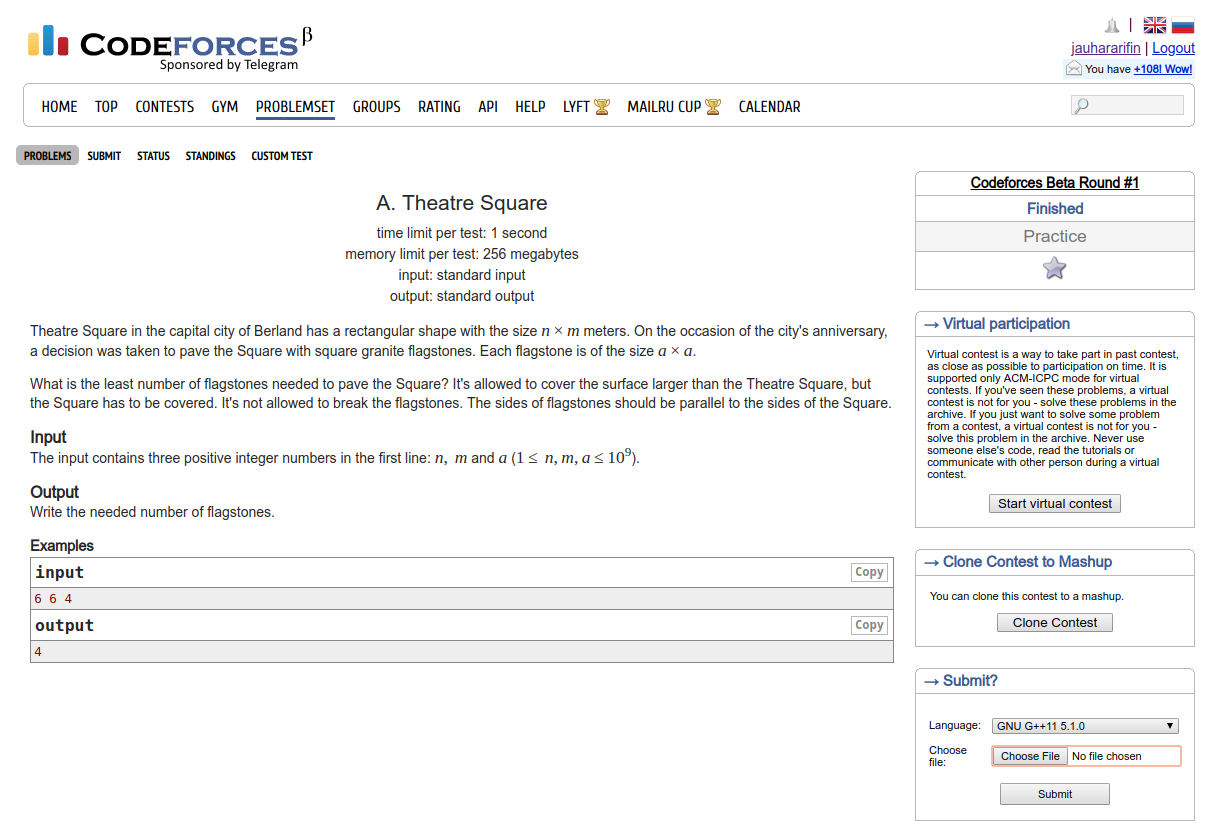
\includegraphics[width=\textwidth]{images/codeforces}
	\caption{Contoh Sistem \textit{Online Judge} : Codeforces.}
	\label{fig:codeforces}
\end{figure}

\par Beberapa organisasi memiliki \textit{online judge} yang secara publik dapat diakses, diantaranya adalah: URI \textit{Online Judge}, TLX, Codeforces, Uva, SPOJ, dan lain sebagainya. \textit{Online judge} yang bersifat publik ini biasanya memiliki beberapa soal-soal yang dapat digunakan untuk latihan dan dapat dikerjakan tanpa harus berkompetisi dengan peserta lain. Pada URI \textit{Online Judge} terdapat fitur tambahan seperti forum dan \textit{rewarding system} (\cite{uriojpaper}). Terdapat beberapa sistem \textit{online judge} yang bersifat \textit{open source} seperti Mooshak, Judgels, dan DomJudge. Sistem \textit{online judge} yang bersifat \textit{open source} biasanya digunakan oleh beberapa instansi seperti perguruan tinggi untuk membuat kompetisi \textit{competitive programming} yang bersifat tertutup seperti Gemastik, Compfest, Vocompfest, Arkavidia, dan INC.

\section{\textit{Autograder}}

\par Pada \textit{competitive programming}, \textit{autograder} merupakan suatu sistem yang digunakan oleh \textit{online judge} untuk melakukan kompilasi, eksekusi dan menilai \textit{source code} (\cite{danutamalms}). \textit{Autograder} digunakan dalam sistem \textit{online judge} untuk menilai kebenaran suatu \textit{source code}. Umumnya \textit{autograder} akan melakukan kompilasi pada \textit{source code} yang dikirimkan oleh peserta pada kompetisi \textit{competitive programming}. Hasil kompilasi dari kode peserta tersebut akan diuji dengan menggunakan \textit{test-case} rahasia yang telah dibuat oleh juri atau \textit{problem setter}. Setelah melalui pengujian, program dinilai kebenarannya berdasarkan hasil pengujian tersebut. Menurut \cite{jordanioi}, cara tersebut disebut sebagai \textit{black-box grading}. Gambar \ref{fig:grading-process} menjelaskan alur penilaian sebuah \textit{source code} yang dikirimkan peserta.

\begin{figure}
	\centering
	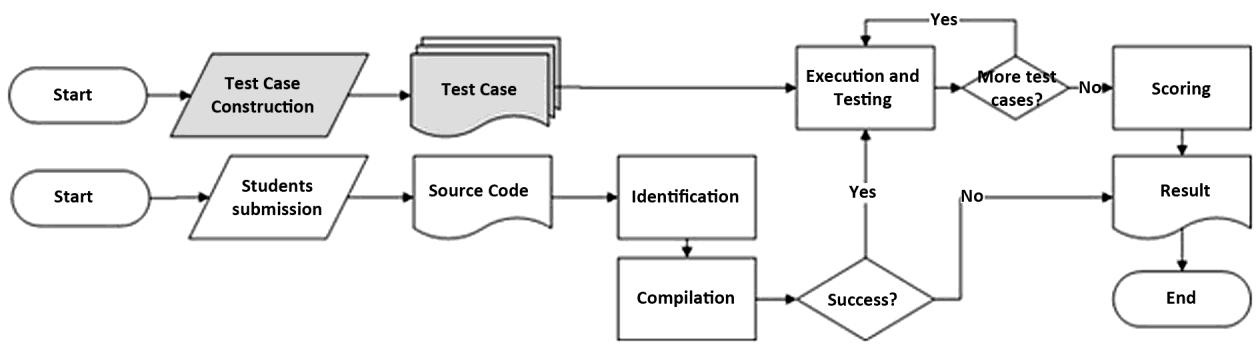
\includegraphics[width=\textwidth]{images/grading-process}
	\caption{Proses penilaian program peserta (\cite{danutamalms})}
	\label{fig:grading-process}
\end{figure}

\par Seluruh proses penilaian sebuah \textit{source code} peserta membutuhkan waktu tiga menit jika dilakukan secara manual, sedangkan hanya membutuhkan waktu sepuluh detik dengan menggunakan \textit{autograder} (\cite{danutamalms}). Dengan menggunakan \textit{autograder}, peserta kompetisi \textit{competitive programming} dapat menerima \textit{feedback} dengan lebih cepat dan mengurangi pekerjaan yang harus dilakukan oleh juri.

\par Dalam menyelenggarakan kompetisi \textit{competitive programming}, juri umumnya menggunakan banyak \textit{autograder} untuk melakukan penilaian jawaban peserta. Dengan menggunakan banyak \textit{autograder}, proses penilaian dapat dilakukan dengan lebih cepat. Untuk menjaga keadilan penilaian, satu buah \textit{autograder} umumnya hanya dapat menilai satu jawaban peserta dalam satu waktu. Jika peserta kompetisi \textit{competitive programming} sangat banyak, maka diperlukan \textit{autograder} yang banyak pula untuk dapat melakukan penilaian jawaban peserta dengan cepat.

\par Terdapat banyak hal yang harus diperhatikan dalam membangun sistem \textit{online judge} dengan menggunakan \textit{autograder}. Salah satu permasalahan yang harus dihadapi dalam membangun \textit{autograder} adalah masalah keamanan sistem. Sistem \textit{autograder} harus dapat bertahan terhadap serangan yang mungkin dilakukan oleh peserta. Beberapa serangan yang mungkin dilakukan oleh peserta adalah mengirimkan \textit{source code} yang memiliki waktu kompilasi yang sangat lama dan membebani sistem, membuat kode yang dapat mengubah atau merusak lingkungan \textit{autograder}, dan mengakses \textit{resource} dari \textit{autograder} yang tidak diizinkan oleh sistem (\cite{wasikojsurvey}). Metode \textit{sandboxing} dapat dilakukan untuk mengatasi masalah keamanan tersebut. \textit{Sandboxing} merupakan teknik untuk mengisolasi suatu eksekusi program sehingga tidak mengganggu lingkungannya. Metode \textit{sandboxing} yang populer pada saat ini antara lain adalah dengan memanfaatkan teknologi \textit{virtualization} seperti KVM, atau teknologi \textit{container} seperti LXC dan Docker.

\par Hal lain yang perlu diperhatikan dalam membangun \textit{autograder} adalah aspek keadilan. Waktu eksekusi program perlu diukur dengan tepat untuk menciptakan sistem yang adil. Waktu eksekusi program yang sama dengan input yang sama dapat memiliki nilai yang berbeda bergantung beberapa faktor seperti kecepatan CPU, ukuran RAM, dan lain sebagainya. Waktu pengukuran sebuah eksekusi program dalam sistem \textit{autograder} biasanya dilakukan dalam hitungan milidetik. Beberapa metode yang dapat digunakan untuk mengukur waktu pemrosesan adalah dengan melakukan analisis pada \textit{hardware performance}, \textit{code instrumentation}, atau \textit{code sampling} (\cite{wasikojsurvey}). Umumnya juri menjaga keadilan penilaian dengan menggunakan spesifikasi komputer yang sama untuk menjalankan banyak sistem \textit{autograder}. Komputer dengan spesifikasi yang sama diharapkan dapat menilai jawaban peserta secara adil.

\section{\textit{Virtual Machine}}

\par \textit{Virtual machine} merupakan teknik \textit{sandboxing} yang memberikan virtualisasi pada tingkat \textit{hardware}. Dengan menggunakan \textit{virtual machine}, pengguna dapat menggunakan komputernya untuk membuat suatu lingkugan yang terisolasi dan seakan-akan merupakan komputer baru yang terpisah dari komputer pengguna. Hal tersebut dapat dilakukan karena adanya \textit{hypervisor} yang digunakan untuk melakukan virtualisasi \textit{hardware} dari suatu komputer. Dengan menggunakan \textit{virtual machine}, pengguna dapat menjalankan lebih dari satu sistem operasi berbeda di dalam komputer yang sama. Pada sistem operasi yang berbasis Linux, terdapat suatu fitur yang bernama KVM yang memungkinkan Linux menjadi \textit{hypervisor} dan menjalankan \textit{guest OS} di dalam proses Linux (\cite{wfeltervmcontainer}).

\par Proses (program yang berjalan) di dalam \textit{virtual machine} terisolasi dari proses yang ada di luar-nya. \textit{Resource} seperti memori dan CPU pada proses di \textit{virtual machine} juga dapat dibatasi. Proses di atas \textit{virtual machine} akan dikelola oleh sistem operasi yang berjalan di \textit{virtual machine} tersebut. Dengan menggunakan KVM, pengguna dapat menjalankan program yang arsitekturnya benar-benar berbeda dengan Linux seperti program berarsitektur Windows. Untuk menjalankan suatu program pada lingkungan \textit{virtual machine}, diperlukan adanya sistem operasi yang mengelola keberjalanan program tersebut. Menjalankan sebuah program pada \textit{virtual machine} dapat menjadi sangat berat karena perlu adanya sistem operasi sendiri yang mengakibatkan adanya pekerjaan tambahan untuk \textit{booting}, manajemen memori, manajemen proses, \textit{scheduling}, dan lain sebagainya.

\par \textit{Virtual machine} tidak cocok untuk digunakan oleh \textit{autograder} karena terlalu banyak pekerjaan tambahan yang diperlukan dan memberatkan sistem. Untuk mengevaluasi \textit{source code} peserta, tidak perlu menggunakan sistem operasi sendiri yang berbeda dengan sistem operasi yang menjalankan sistem \textit{autograder}. \textit{Virtual machine} lebih cocok digunakan untuk melakukan pengujian program yang membutuhkan berbagai macam jenis sistem operasi. Selain itu, \textit{virtual machine} juga kerap digunakan dalam pembuatan sistem IaaS (\textit{Infrastructure as a service}) seperti Amazon EC2, Digital Ocean Droplet dan Google Cloud Compute Engine.

\section{\textit{Containerization}}

% TODO: enrich this, jelasin rlimit, signal, capabilities, setuid

\par Secara singkat, \textit{container} merupakan teknologi virtualisasi proses pada tingkat sistem operasi. Teknik \textit{containerization} berbeda dengan teknik virtualisasi menggunakan \textit{hypervisor} yang bekerja pada tingkat \textit{hardware} (\cite{merkeldocker}). \textit{Container} bekerja seperti \textit{virtual machine} yang dapat memberikan isolasi terhadap program yang berjalan. Pada \textit{virtual machine}, virtualisasi terjadi pada tingkat \textit{hardware} sehingga pengguna perlu memasang sistem operasi pada lingkungan yang terisolasi untuk dapat menjalankan program. Pada \textit{container}, pengguna tidak perlu memasang sistem operasi karena virtualisasi terjadi pada tingkat \textit{software} sehingga sistem operasi yang berjalan pada komputer pengguna dapat digunakan di dalam \textit{container}. Hal tersebut membuat \textit{container} lebih ringan dibandingkan \textit{virtual machine} karena tidak ada kerja tambahan untuk menjalankan sistem operasi baru.

\par Pada Linux, teknologi \textit{container} mungkin dilakukan karena adanya beberapa fitur dari Linux yaitu: \textit{chroot}, \textit{cgroup} dan \textit{namespace}. \textit{Chroot} dapat memberikan isolasi \textit{file system} terhadap suatu proses pada Linux. \textit{Cgroup} dapat memberikan batasan \textit{resource} kepada suatu proses di Linux. \textit{Namespace} dapat memberikan isolasi pada proses sehingga proses dalam suatu lingkungan tidak dapat mengetahui adanya proses lain di lingkungan yang berbeda. Terdapat beberapa perangkat lunak yang menawarkan teknologi \textit{containerization} ini, yang populer diantaranya adalah Docker dan LXC. Dengan menggunakan Docker atau LXC, pengguna dapat membuat suatu lingkungan yang tersiolasi untuk menjalankan suatu program tertentu tanpa mengganggu lingkungan di luar-nya. Docker memberikan API yang lebih \textit{high-level} dibandingkan dengan LXC, dan memiliki banyak fitur yang dapat digunakan untuk mengelola \textit{container}. Docker sudah banyak digunakan sebagai \textit{platform} untuk menjalankan dan mendistribusikan aplikasi.

\par Teknologi \textit{container} ini dapat digunakan untuk melakukan penilaian terhadap kode program yang dikirimkan oleh peserta kompetisi \textit{competitive programming}. Dengan menggunakan \textit{container}, program yang dijalankan dapat diisolasi sehingga tidak membahayakan lingkungan di luar-nya. Selain itu, \textit{resource} seperti CPU, memori, \textit{storage}, dan IO pada \textit{container} dapat dibatasi sehingga tidak mengganggu program lain yang sedang berjalan pada lingkungan di luar \textit{container} (\cite{merkeldocker}).

\subsection{\textit{Chroot}}

\par \textit{Chroot} merupakan \textit{system call} pada sistem operasi yang berbasis Linux atau Unix. \textit{System call} ini dapat mengubah \textit{root file system} dari suatu proses ke direktori target tertentu. Program yang dijalankan seakan-akan memiliki direktori \textit{root} sebagai direktori yang ditentukan pada waktu pemanggilan \textit{system call} \textit{chroot}. Dengan menggunakan cara ini, program yang dijalankan dalam \textit{chroot} hanya dapat mengakses \textit{file system} yang berada pada direktori target saja dan mengurangi kemungkinan serangan yang mungkin dilakukan pada \textit{file system} asli (\cite{lessardchroot}). Dengan menggunakan \textit{chroot}, pengguna dapat mengatur \textit{library} apa saja yang dapat digunakan oleh program yang berjalan dalam lingkungan \textit{chroot}. Hal ini dapat menjadi merepotkan karena pengguna perlu memasukkan semua \textit{library} yang dibutuhkan ke dalam \textit{file system} \textit{chroot}. Teknologi \textit{container} memanfaatkan \textit{chroot} untuk mengisolasi \textit{file system} yang dapat diakses oleh program yang berjalan pada \textit{container}.

\par Meskipun \textit{chroot} memberikan penghalang pada aplikasi yang berada dalam lingkungan \textit{chroot} untuk mengakses \textit{file system} yang berada di luar lingkungan direktori target, \textit{chroot} masih memiliki kelemahan. Jika aplikasi yang berjalan pada lingkungan \textit{chroot} memiliki \textit{root permission}, maka aplikasi tersebut dapat dengan mudah keluar dari lingkungan \textit{chroot}. Terdapat beberapa cara untuk meningkatkan keamanan \textit{chroot} sehingga program yang berjalan di dalam \textit{chroot} sulit  untuk keluar dari lingkungan tersebut.

\par Salah satu cara untuk meningkatkan keamanan pada lingkungan \textit{chroot} adalah dengan memasukkan file yang hanya dibutuhkan oleh program saja. Sebagai contoh, jika program membutuhkan daftar \textit{user} yang berada dalam sistem, di dalam linkungan \textit{chroot} perlu ada file /etc/passwd untuk mendapatkan informasi ini. Akan tetapi, file /etc/shadow tidak perlu dimasukkan ke dalam \textit{file system} \textit{chroot} karena mengandung informasi rahasia yang tidak diperlukan oleh program yang berada dalam lingkungan \textit{chroot}.

\par Cara kedua untuk meningkatkan keamanan lingkungan \textit{chroot} adalah dengan tidak memberikan akses \textit{root} kepada program yang berjalan di dalam \textit{chroot}. Terdapat beberapa serangan yang memungkinkan program dalam lingkungan \textit{chroot} untuk keluar dari lingkungan \textit{chroot} jika memiliki akses \textit{root}. Untuk menghindari jenis serangan ini, sebaiknya program yang berjalan di dalam lingkungan \textit{chroot} dibuat agar tidak mungkin mendapatkan akses \textit{root}. Tidak memberikan akses \textit{root} kepada program akan mengurangi kemungkinan adanya serangan. Akan tetapi, meskipun tidak memberikan akses \textit{root}, masih terdapat beberapa serangan yang memungkinkan program membangkitkan akses \textit{root} tanpa memiliki akses \textit{root} pada saat dijalankan.

\par Untuk meningkatkan keamanan pada lingkungan \textit{chroot}, sebaiknya tidak memasukkan \textit{hard link} ke dalam \textit{file system} \textit{chroot}. \textit{Hard link} yang mengacu pada file di luar lingkungan \textit{chroot} akan mengurangi keamanan \textit{chroot} karena memungkinkan program yang berada di dalam lingkungan \textit{chroot} untuk mengakses file yang berada di luar lingkungan \textit{chroot}.

\subsection{\textit{Cgroup}}

% TODO: jelasin hirarki cgroup

\par \textit{Cgroup} merupakan fitur pada Linux yang dapat digunakan untuk membatasi \textit{resource} yang digunakan oleh suatu kelompok program (\cite{wfeltervmcontainer}). \textit{Resource} yang dimaksud di sini adalah \textit{CPU usage}, \textit{memory usage} dan \textit{disk IO}. Dengan menggunakan \textit{cgroup}, sebuah program yang dibatasi \textit{resource}-nya tidak akan mengganggu program lain dengan cara menghabiskan \textit{resource}. Fitur \textit{cgroup} dimanfaatkan oleh teknologi \textit{container} untuk membatasi \textit{resource} pada sebuah \textit{container} sehingga tidak membebani program lain di luar \textit{container}. Pada \textit{container}, umumnya \textit{cgroup} digunakan untuk membatasi CPU dan memori yang digunakan oleh program-program yang berjalan di dalam \textit{container}. \textit{Cgroup} dapat memberhentikan program di dalam \textit{container} jika telah menggunakan \textit{resource} yang berlebihan. Selain itu, \textit{cgroup} juga dapat digunakan untuk mengukur penggunaan resource oleh suatu proses yang berjalan pada komputer. Hal tersebut dapat digunakan untuk mengukur waktu eksekusi program peserta.

\subsection{\textit{Namespace}}

\par Dengan menggunakan \textit{chroot} dan \textit{cgroup}, sebuah program dapat diisolasi sehingga memiliki \textit{resource} dan \textit{file system} sendiri yang terpisah dari program-program lain yang berjalan pada sistem operasi \textit{host}. Yang dimaksud sistem operasi \textit{host} disini adalah sistem operasi yang digunakan oleh pengguna tanpa adanya isolasi \textit{container}. Meskipun \textit{resource} dan \textit{file system} dari proses sudah berhasil diisolasi, proses ini masih dapat melihat proses apa saja yang sedang berjalan pada sistem operasi \textit{host} karena program yang berjalan di dalam \textit{chroot} dan \textit{cgroup} masih menggunakan sistem operasi yang sama dan menggunakan \textit{kernel} yang sama. Linux memiliki fitur \textit{namespace} yang memberikan isolasi kepada proses terhadap proses lain pada lingkungan yang berbeda. Dengan menggunakan \textit{namespace}, sebuah proses di suatu \textit{namespace} tertentu dan hanya dapat mengetahui proses lain yang berada di dalam \textit{namespace} yang sama. \textit{Container} memanfaatkan \textit{namespace} sehingga program yang berjalan di dalam \textit{container} hanya mengetahui proses lain yang berada di dalam \textit{container} tersebut dan tidak dapat mengetahui proses pada sistem operasi \textit{host}-nya (\cite{wfeltervmcontainer}).

\par Selain isolasi program, \textit{namespace} juga memberikan isolasi pada hal lain seperti \textit{network}, \textit{mount}, \textit{cgroup}, \textit{user}, dan lain sebagainya. Dengan memberikan isolasi pada \textit{network}, program yang berada di dalam \textit{container} dapat membuka \textit{port} yang sama seperti program lain yang berada di \textit{container} lain. Dengan menggaunakan isolasi pada \textit{user}, \textit{user} yang ada di dalam \textit{container} tidak dapat diketahui oleh \textit{container} lain.

\section{WebAssembly}

\par WebAssembly merupakan API \textit{Web} yang memungkinkan \textit{browser} untuk menjalankan \textit{low-level code} secara aman. Dulunya Javascript merupakan satu-satunya bahasa yang didukung secara \textit{native} oleh \textit{web}, akan tetapi semakin berkembangnya teknologi \textit{web} kebutuhan akan kinerja dari \textit{web} semakin tinggi. Javascript yang merupakan \textit{interpreted language} tidak dapat memberikan kinerja yang tinggi seperti bahasa-bahasa yang dikompilasi menjadi \textit{low-level code}. WebAssembly memberikan solusi yang memungkinkan \textit{browser} untuk menjalankan \textit{low-level code} pada sebuah sistem yang terisolasi dan aman. WebAssembly didesain untuk digunakan bersama-sama dengan Javascript untuk mengembangkan aplikasi \textit{web}. Sebuah aplikasi \textit{web} dapat memanfaatkan WebAssembly untuk meningkatkan kinerja dan memanfaatkan Javascript untuk fleksibilitas (\cite{mdnwebasm}).

\par Dengan menggunakan WebAssembly, \textit{browser} dapat membuat sebuah lingkungan yang terisolasi untuk menjalankan \textit{low-level code}. Lingkungan yang digunakan untuk menjalankan kode WebAssembly memiliki beberapa batasan seperti jumlah memori yang bisa digunakan, \textit{file} yang bisa diakses dan lain sebagainya. Umumnya kode WebAssembly hanya dapat melakukan apa yang dapat dilakukan oleh \textit{web}. \textit{Web} tidak dapat mengakses sembarang \textit{file} yang berada pada komputer, begitu juga dengan WebAssembly. \textit{Web} tidak dapat melakukan beberapa \textit{system call}, begitu juga WebAssembly. Meskipun WebAssembly dapat memberikan isolasi pada program yang berjalan, pembatasan \textit{resource} pada WebAssembly masih sulit dilakukan dan tidak semudah pembatasan \textit{resource} pada \textit{container} ataupun \textit{virtual machine}. 

\par Kode WebAssembly berupa \textit{binary code} yang dapat dibuat dengan cara melakukan kompilasi dari beberapa bahasa seperti C, C++ dan Rust ke dalam format \textit{wasm}. WebAssembly masih baru dan belum banyak bahasa pemrograman yang dapat dikompilasi menjadi WebAssembly. Bahasa pemrograman yang menggunakan \textit{interpreter} atau \textit{runtime environment} seperti Python dan Java masih sulit dijalankan di dalam WebAssembly.

\par Dalam sistem \textit{autograder}, WebAssembly tidak cocok digunakan karena berbagai alasan, yaitu: masih sedikitnya bahasa pemrograman yang dapat dikompilasi menjadi kode WebAssembly, sulitnya membatasi \textit{resource} pada WebAssembly, sulitnya melakukan perhitungan waktu, dan sulitnya menjaga keamanan. \textit{Browser} yang ada pada saati ini memiliki kemampuan untuk mengubah kode Javascript yang berjalan pada \textit{browser} tersebut, hal ini mengakibatkan munculnya celah keamanan pada WebAssembly jika digunakan untuk mengevaluasi kode peserta.
